\documentclass[conference]{IEEEtran}
\usepackage[T1]{fontenc}
\usepackage{amsmath,amssymb,bm,booktabs,graphicx,cite}
\usepackage[hidelinks]{hyperref}
\newcommand{\E}{\mathbb{E}}
\newcommand{\R}{\mathbb{R}}
\newcommand{\C}{\mathbb{C}}
\newcommand{\pos}[1]{[#1]_+}
\newcommand{\norm}[1]{\lVert#1\rVert}
\newcommand{\G}{\mathsf{G}}
\newcommand{\SIC}{\mathsf{S}}
\newcommand{\Sel}{\mathsf{Select}}
\newcommand{\DraftNotice}{}
\newcommand{\ResultFigure}[1]{\includegraphics[width=\columnwidth]{#1}}

\title{Blind Disturbance-Model Selection for\\Diffusion-Aided Semantic Image Reception}
\author{\IEEEauthorblockN{Author information pending}
\IEEEauthorblockA{Affiliations and correspondence to be supplied}}
\begin{document}
\maketitle
\begin{abstract}
Explicit interference reconstruction is useful only when its additional
modeling assumptions improve the desired image estimate. With unknown
interference power, a joint diffusion sampler may instead introduce errors
and unnecessary computation. We propose a blind disturbance-model selector
for a frozen semantic image codec. Before diffusion inference, the receiver
uses excess received energy and block-energy heterogeneity to choose either
Gaussian denoising or joint signal--interference reconstruction. The rule is
fitted on separate development images; only the selected branch is executed,
and no neural weights are updated. We evaluate the rule on CelebA images with
CIFAR-10 interference, using identical received signals for all receiver
comparisons and a joint receiver with the same bypass as an additional control.
On 256 independent image pairs with two random seeds and 18 channel conditions, the frozen rule reaches 21.593 dB mean PSNR. It improves on calibrated joint sampling by +1.334 dB and on blind Gaussian denoising by +0.750 dB. The rule uses 52.2 predictor evaluations per frame on average, compared with 80 for joint sampling.

Separately trained DeepJSCC and MambaJSCC codecs provide external performance
references under the same channel-use budget.
\end{abstract}
\begin{IEEEkeywords}
Semantic communications, interference cancellation, diffusion models,
receiver adaptation, deep joint source--channel coding.
\end{IEEEkeywords}
\DraftNotice

\section{Introduction}
Deep joint source--channel coding (JSCC) maps an image directly to channel
symbols, allowing the decoder to learn robustness to transmission noise
\cite{bourtsoulatze2019deep,yang2025swinjscc}. A deployed codec can nevertheless
encounter co-channel interference absent from its training channel. Diffusion
priors offer two ways to process the received symbols. Channel denoising
diffusion models (CDDM) motivate treating the disturbance as Gaussian
\cite{wu2024cddm}, whereas interference cancellation diffusion models (ICDM)
represent the desired and interfering signals explicitly \cite{wu2026icdm}.

The more detailed model is not always the better receiver. Gaussian denoising
ignores interference structure but avoids estimating a second latent signal.
Joint reconstruction uses that structure, at the cost of estimating both the
interferer and its unknown amplitude from one mixture. Errors in those estimates
can degrade the desired image even when the reconstructed mixture fits the
observation. A fixed choice therefore risks either discarding useful structure
or paying for unreliable separation.

We address the resulting decision: \emph{when should a frozen receiver denoise
the aggregate disturbance, and when should it reconstruct the interferer?}
The decision must precede diffusion inference. Running both receivers and
choosing the better reconstruction would require an unavailable quality
reference and incur both inference costs. Our selector instead computes two
statistics from the received symbols: excess energy estimates disturbance
strength, while block-energy heterogeneity describes variation across symbol blocks.
A threshold rule learned on separate development images selects one branch.
The codec and both diffusion priors remain frozen.

The contribution has three parts:
\begin{itemize}
\item a blind selection rule that chooses the disturbance model before sampling,
using $O(n)$ received-energy calculations and no additional neural inference;
\item a development-only fitting procedure that compares energy-only and
two-feature rules, and retains a fixed receiver when validation finds no gain;
\item an independent paired evaluation that separates model selection from
power estimation and direct-decoding bypass, and measures both reconstruction
gains and harmful decisions.
\end{itemize}
The key comparison is against a Gaussian receiver calibrated to \emph{total}
disturbance, not thermal noise alone. A joint receiver with the same bypass
provides a second control for improvements caused merely by skipping
separation. These controls test the receiver decision without changing the
underlying learned representations.

\section{Related Work}
CDDM matches channel noise to a diffusion noise level and jointly considers
codec training, channel denoising and decoder adaptation \cite{wu2024cddm}.
ICDM adds an interference prior for joint signal recovery \cite{wu2026icdm}.
We use these two receiver principles with shared frozen weights to study their
selection. The resulting Gaussian and joint receivers are receiver-only ports;
they do not reproduce the complete published training pipelines.
DeepJSCC \cite{bourtsoulatze2019deep}, SwinJSCC \cite{yang2025swinjscc}, and
MambaJSCC \cite{wu2024mambajscc} provide the codec context for our experiments.
The separately trained direct-codec references in Section IV locate the
reported quality relative to other architectures.

Other methods adapt reconstruction within an inference procedure. ISEC
iteratively corrects latent errors using a learned source prior
\cite{pmlr-v206-lee23c}. DiffCom conditions generative reconstruction on channel
observations and includes blind inference of transmission characteristics
\cite{wang2025diffcom}. GibbsDDRM estimates unknown forward-model parameters
during diffusion inference \cite{murata2023gibbsddrm}. Our decision occurs
before such iterative processing: it selects which disturbance treatment to
invoke. We study the usefulness and cost of that choice, without proposing a
new diffusion prior or posterior inference algorithm.

\section{System Model and Receiver Choice}
\subsection{An Interfering Latent Transmission}
Let $\bm u\in[0,1]^d$ be the desired image, and let the frozen encoder produce
$\bm x\in\C^n$. A separate transmitter produces interfering symbols
$\bm z\in\C^n$. Each transmitter normalizes its frame to unit average complex
symbol power. The additive channel is
\begin{equation}
 \bm y_b=\bm x_b+a_b\bm z_b+\bm w_b,\qquad
 \bm w\sim\mathcal{CN}(\bm0,N_0\bm I),\quad a_b\ge0 ,
 \label{eq:channel}
\end{equation}
where $b$ indexes $B$ contiguous blocks, with $L_b$ complex symbols per
block. The channel bandwidth ratio is
$n/d$. The receiver knows $N_0$, the normalization convention, and a chosen
block partition, but not $a_b$, the interference profile, $\bm z$, or $\bm u$.
The test channel has unit desired-channel gain. Fading, channel estimation, and
synchronization are outside this experiment.

For a prescribed nominal SINR $\gamma$, the simulator sets average nominal
interference power to $10^{-\gamma/10}-N_0$. The instantaneous interference
energy also depends on the realized block energies of $\bm z$; nominal SINR
must therefore not be confused with measured per-frame SINR.

The explicit model associates two learned priors with \eqref{eq:channel}:
\begin{equation}
 \begin{split}
 p(\bm x,\bm z\mid\bm y,\bm a)&\propto p_s(\bm x)p_z(\bm z)\\
 &\quad\times\exp\!\left[-\frac{1}{N_0}\sum_b
 \norm{\bm y_b-\bm x_b-a_b\bm z_b}^{2}\right].
 \end{split}
 \label{eq:joint}
\end{equation}
This equation describes the model; our finite-step sampler is an approximation,
not an exact posterior draw or a proven MAP optimizer.
Without priors, the change
$\bm x_b'=\bm x_b+a_b\bm\delta_b$,
$\bm z_b'=\bm z_b-\bm\delta_b$ leaves the mixture unchanged.
Power constraints remove some ambiguity but do not generally identify both
latents. The Gaussian model instead uses
\begin{equation}
 p_{\G}(\bm y\mid\bm x;\nu)=
 \mathcal{CN}(\bm y;\bm x,\nu\bm I),\qquad \nu\ge N_0 .
 \label{eq:gaussian}
\end{equation}
It sacrifices interference structure to avoid explicit component estimation.

\subsection{Two Frozen Candidate Receivers}
Both candidates process the same received frame and use the same desired-signal
prior and decoder. They differ in how they represent the disturbance.
For Gaussian reception, estimate the disturbance from raw received symbols:
\begin{equation}
 \begin{gathered}
 e_b=\frac{\norm{\bm y_b}^2}{L_b},\qquad
 \bar e=\frac{1}{n}\sum_b L_be_b,\\
 \widehat P=\pos{\bar e-1-N_0},\qquad
 \widehat\nu=N_0+\widehat P.
 \end{gathered}
 \label{eq:energy}
\end{equation}
With unit source power and vanishing signal--interference cross expectation,
unclipped excess energy estimates mean interference energy. Finite blocks,
latent correlations, and clipping prevent treating it as an exact amplitude
estimate. In particular, local desired-signal energy can resemble interference
heterogeneity.

Let $r(\bm y)\in\R^{2n}$ stack real and imaginary components. Given the training
diffusion schedule $\bar\alpha_t$, the Gaussian receiver $\G$ starts at the
nearest noise level satisfying
\begin{equation}
 \frac{1-\bar\alpha_{t_0}}{\bar\alpha_{t_0}}
 \simeq\frac{\widehat\nu}{2},\qquad
 \bm v_{t_0}=\sqrt{\bar\alpha_{t_0}}\,r(\bm y).
 \label{eq:match}
\end{equation}
The factor $1/2$ converts complex noise power to variance per real coordinate.
For decreasing respaced indices, a noise predictor $\epsilon_s$ gives
\begin{align}
 \widehat{\bm x}_0&=
 \frac{\bm v_t-\sqrt{1-\bar\alpha_t}\epsilon_s(\bm v_t,t)}
 {\sqrt{\bar\alpha_t}},\\
 \bm v_{t'}&=\sqrt{\bar\alpha_{t'}}\widehat{\bm x}_0+
 \sqrt{1-\bar\alpha_{t'}}\epsilon_s(\bm v_t,t).
 \label{eq:gaussian_update}
\end{align}
At most 40 predictor evaluations are used, with fewer when the matched initial
index is below 39. A common normalization and the frozen decoder produce the
reconstructed image.

The structured receiver $\SIC$ initializes
$a_b^{(0)}=\sqrt{\pos{e_b-1-N_0}}$ and performs joint diffusion inference with
signal and interference predictors. During late corrector updates it obtains
denoised, frame-normalized estimates $\widetilde{\bm x}$ and
$\widetilde{\bm z}$, then updates
\begin{equation}
 a_b^{+}=\pos{\frac{
 \Re\{\widetilde{\bm z}_b^{H}
       (\bm y_b-\widetilde{\bm x}_b)\}}
 {\norm{\widetilde{\bm z}_b}^{2}}}.
 \label{eq:amplitude}
\end{equation}
An empty denominator retains the previous amplitude. This is a nonnegative
least-squares update conditional on point estimates, not a correction for
their uncertainty. Calibration begins when the signal coefficient
$\alpha(t)\ge0.5$. Estimated block SINR updates the inherited guidance
coefficients by clipped linear interpolation of the original AWGN table.
We use the existing 40-step, order-three joint sampler: 40 signal and 40
interference evaluations. The initialization-only variant keeps amplitudes
fixed and supplies an ablation of calibration.

\subsection{Selection Before Generative Inference}
The selector augments $\widehat P$ with normalized block-energy variation
\begin{equation}
 H=\frac{B^{-1}\sum_{b=1}^{B}(e_b-\bar e)^2}
          {\max(\bar e^2,\varepsilon)}.
 \label{eq:heterogeneity}
\end{equation}
Here $\varepsilon>0$ prevents division by zero, and all receiver blocks have
equal length. $H$ measures energy variation, not the interference distribution. For
$\theta=(\tau_\ell,\tau_h,\eta)$, define
\begin{equation}
 \pi_\theta(\bm y)=
 \begin{cases}
 \G,&\widehat P\le \tau_\ell,\ H\le\eta,\\
 \G,&\widehat P\le \tau_h,\ H>\eta,\\
 \SIC,&\text{otherwise}.
 \end{cases}
 \label{eq:selector}
\end{equation}
We also test the reversed assignment of $\G$ and $\SIC$ in
\eqref{eq:selector}; the Gaussian branch is not assumed to belong to the
low-power region. The energy-only family sets $\tau_\ell=\tau_h$. Either family can reduce to a
constant receiver; heterogeneity need not be useful.

We fit thresholds to mean per-image PSNR on development data. Eight folds keep
all channel conditions belonging to one image together. Each fold is predicted
using thresholds fitted on the other seven, then the family with the highest
out-of-fold mean is refitted on all development images. Ties prefer lower
component inference cost and then the simpler family. If neither family
improves on the better fixed receiver in development validation, that fixed
receiver is retained. No threshold is adjusted using confirmation or pressure
results. At reception, \eqref{eq:selector} is computed first and only its chosen
branch is executed. Selection adds $O(n)$ energy calculations and no diffusion
evaluations.

For analysis, let $q_j(\bm u,\bm y)$ be a candidate's PSNR. The unavailable
per-frame oracle has quality $\max(q_\G,q_\SIC)$. The exact identity
\begin{equation}
 \max(q_\G,q_\SIC)-q_{\pi_\theta}
 =|q_\G-q_\SIC|\,
 \mathbf1\{\pi_\theta\ne\arg\max_j q_j\}
 \label{eq:regret}
\end{equation}
shows that complementary receivers are necessary but not sufficient: mistakes
on large-gap frames matter most. This is an accounting identity, not a
generalization bound. Mean PSNR is the fitting objective; neither mean MSE,
LPIPS nor harmful-tail probability is implicitly optimized.

\section{Experimental Evaluation}
\subsection{Data, Receivers, and Evaluation Protocol}
The desired images are $128\times128$ center crops from CelebA
\cite{liu2015celeba}. CIFAR-10 interference images are cropped at
$32\times32$ and nearest-neighbor upsampled to the encoder input size.
The original training sets contain 162,770 desired and 50,000 interference
images. The inherited codec uses three Swin stages with widths
$(128,192,256)$ and depths $(2,2,6)$; its 8-channel $16\times16$ real latent
corresponds to 1,024 complex symbols and CBR $1/48$.
Five frozen checkpoints contain the desired encoder/decoder, interference
encoder, and two DiT predictors, each with 28 blocks, width 1,152, 16 heads
and patch size two. The original frozen-study training schedule uses
100 interference-codec epochs, 40 desired-codec epochs, and 50/20 epochs for
the signal/interference predictors. The selector study adds no neural
retraining. The two direct codec anchors are separately retrained for 40 epochs
at SNR 20 dB with 1,024 complex channel uses (CBR $1/48$); each also trains a
matched CIFAR-10 interference encoder. Best checkpoints minimize held-out
validation MSE; training uses one seed. DeepJSCC uses a pinned third-party
PyTorch reproduction, while MambaJSCC uses its official repository. We
also test transfer using
repository-released weights without fine-tuning. Public
MambaJSCC retains CBR $1/48$ but differs in training domain, channel and
resolution; the available DeepJSCC weight uses CBR $0.16256$. These
protocol-mismatched diagnostics use the same public encoder for both image
streams and are reported separately from the retrained references.

Development uses 64 validation image pairs and seed 1700. Confirmation reserves
256 previously unevaluated test pairs with seeds 2700 and 2701.
SNR is 20 dB; nominal SINR is $-7,-4,0,4,7,10$ dB.
Sixteen blocks of 64 complex symbols follow stationary, alternating
$(0.25,1.75)$, or burst $(0,2)$ relative-power patterns.
Each pair is evaluated under all 18 conditions.
The confirmation set therefore has 9,216 received frames but only 256
image-pair clusters. Confirmation starts only after policy fitting ends.
File-hash audits exclude overlap with development, pressure images and the
first 200 test pairs used in earlier project evaluations. The independence
claim is at image-pair level, not at person-identity level.

We compare direct decoding; the same Gaussian port using only $N_0$;
the blind-total-disturbance Gaussian receiver $\G$; initialization-only joint
sampling; calibrated joint sampling $\SIC$; and the online selector.
A same-gate control decodes directly when $\widehat P\le0.15$ and otherwise uses
$\SIC$. Its output quality is reconstructed exactly from paired branches;
its reported cost excludes gate overhead. Development additionally examines
the previous coupled-feedback receiver and a Gaussian port given nominal
total disturbance power. The nominal-power receiver is a privileged development diagnostic, not a
guaranteed upper bound.
DeepJSCC and MambaJSCC direct decoding are reported as absolute anchors using
their own desired and interference codewords under the same channel grid.
The diffusion priors are specific to the SwinJSCC latent distribution;
attaching them to another codec would require new prior training. Reproducing
complete CDDM/ICDM training and decoder adaptation remains outside this
receiver study, so published-system competitiveness remains unestablished.

The prespecified power thresholds are
$0$, $0.1$, $0.2$, $0.35$, $0.5$, $0.75$, $1$, $1.5$, $2$, $3$, $4$, $8$ and $10^6$;
heterogeneity thresholds are $\{0.05,0.1,0.2,0.4,0.8,1.6\}$.
Including both assignment directions, the families contain 26 and 2,028
candidate rules.
All SwinJSCC receiver variants see identical received tensors. The two direct
anchors use separately encoded, unit-power codewords at the same budget and
reuse the image pairs, conditions, and channel seeds. Channel randomness is
separate from sampler randomness; both CPU and GPU sampler states are reset per
frame.
Measurements use float32, batch one, TF32 disabled, four CPU threads, and one
RTX 4090. Synchronized receiver time includes selection, sampling and decoding,
but excludes encoding, image-quality evaluation and one-time model loading.
Signal and interference model calls are counted separately.

We report arithmetic means of per-image PSNR and MSE, LPIPS-VGG v0.1
\cite{zhang2018lpips}, and four-scale MS-SSIM
\cite{wang2003msssim}, always clipping RGB to $[0,1]$.
Four scales fit the image resolution; these values are not compared with
five-scale scores. Paired 95\% intervals resample image-pair clusters 5,000
times while retaining both seeds and all conditions. Harm means a PSNR loss
exceeding 0.5 dB relative to a specified comparator. The resampling unit is the image pair rather than individual frames.

\subsection{Frozen Rule and Receiver Comparison}
Image-group validation compares the two rule families. Energy-only selection yields 22.002 dB, whereas the two-feature family yields 22.239 dB. We therefore retain the energy and heterogeneity rule with $\tau_\ell=8$, $\tau_h=0.5$ and $\eta=0.2$, with Gaussian reception below the applicable power threshold.

The low-heterogeneity development region contains 810 frames and has a maximum excess-energy estimate of 5.241. The fitted threshold 8 therefore lies beyond observed support and makes this region always Gaussian. This threshold is not an identified physical transition, and the family comparison does not establish that either feature is individually necessary. The earlier coupled-feedback receiver obtains 20.477 dB, versus 20.605 dB for calibrated joint sampling and 20.835 dB for its same-gate control. The privileged nominal-power Gaussian diagnostic obtains 21.591 dB. These development comparisons motivate the receiver decision but are not independent confirmation.

Table~\ref{tab:main} and Fig.~\ref{fig:quality} report the independent experiment. The selector changes mean PSNR by +1.334 dB relative to calibrated joint sampling (95\% interval [1.265, 1.404]), +0.750 dB relative to blind Gaussian denoising (95\% interval [0.698, 0.806]), and +1.140 dB relative to the same-gate control (95\% interval [1.075, 1.205]). Both fixed-receiver comparisons have positive paired intervals, supporting a mean-PSNR benefit within the matched confirmation population. Estimating total disturbance changes the Gaussian receiver from 18.829 to 20.843 dB, so the thermal-noise-only port is insufficient as the sole Gaussian baseline. Disaggregating blind Gaussian/joint/selector PSNR gives stationary 21.310/19.282/21.317 dB with 98.8\% Gaussian choices, alternating 20.737/20.178/21.285 dB with 59.5\% Gaussian choices, burst 20.481/21.317/22.177 dB with 50.1\% Gaussian choices. This profile dependence is consistent with complementary receiver utility, but does not identify the physical cause of the heterogeneity statistic.

\begin{table}[t]
\centering
\caption{Independent confirmation. Quality is averaged per image and frame.
NFE counts both priors; latency is synchronized batch-one receiver time.
The same-gate control's latency is a component estimate. DeepJSCC and
MambaJSCC rows are matched-retrained direct-codec anchors; all remaining
rows share the frozen SwinJSCC codec.}
\label{tab:main}
\scriptsize\setlength{\tabcolsep}{2.4pt}
\begin{tabular}{lrrrrrr}
\toprule
Receiver & PSNR & MSE$\times10^3$ & LPIPS & MS-SSIM & NFE & ms\\
\midrule
SwinJSCC direct & 18.67 & 29.14 & 0.440 & 0.697 & 0.0 & 8\\
DeepJSCC direct & 17.39 & 24.71 & 0.575 & 0.684 & 0.0 & 1\\
MambaJSCC direct & 16.92 & 44.13 & 0.463 & 0.613 & 0.0 & 10\\
Gaussian (N0) & 18.83 & 28.70 & 0.438 & 0.700 & 18.0 & 225\\
Blind Gaussian & 20.84 & 24.90 & 0.378 & 0.782 & 40.0 & 488\\
Init. joint & 19.61 & 20.15 & 0.363 & 0.793 & 80.0 & 1110\\
Calibrated joint & 20.26 & 18.49 & 0.362 & 0.802 & 80.0 & 1180\\
Joint + gate & 20.45 & 18.43 & 0.361 & 0.801 & 65.9 & 974\\
Selector & 21.59 & 16.45 & 0.336 & 0.832 & 52.2 & 701\\
\bottomrule
\end{tabular}

\end{table}
\begin{figure}[t]
\centering
\ResultFigure{figures/confirmation_quality.pdf}
\caption{Independent confirmation by nominal SINR, averaging all three
interference profiles. Solid curves compare receivers in the frozen SwinJSCC
latent space; dashed curves are separately retrained direct-codec anchors.}
\label{fig:quality}
\end{figure}

\subsection{Inference Cost and Harmful Decisions}
The selector chooses Gaussian reception on 69.5\% of confirmation frames. Its average cost is 52.2 predictor evaluations and 701 ms, versus 80 evaluations and 1180 ms for joint sampling. Against that receiver, 3.79\% of frames lose more than 0.5 dB, and the fifth percentile of the paired change is -0.127 dB (Fig.~\ref{fig:tail}). The unavailable per-frame oracle reaches 21.760 dB; selection leaves 0.167 dB mean oracle regret. Mean MSE changes from 0.01849 to 0.01645, LPIPS from 0.3618 to 0.3362, and MS-SSIM from 0.8015 to 0.8318. These secondary metrics and the harmful tail must accompany the average PSNR comparison.

\begin{figure}[t]
\centering
\ResultFigure{figures/paired_tail.pdf}
\caption{Paired PSNR change on independent confirmation relative to calibrated
joint sampling. Each point in the empirical CDF represents one received
frame; uncertainty calculations cluster by image pair. The vertical line
marks the predefined harmful-loss threshold.}
\label{fig:tail}
\end{figure}

\subsection{Block Mismatch and No Interference}
Pressure tests use 64 further test pairs and seed 3700, with nominal SINR
$-4,4,10$ dB. One profile shifts burst boundaries by half a receiver block;
another draws segment lengths uniformly from 16 to 128 symbols and normalizes
the binary on/off amplitude pattern. A separate SNR-20 condition has no
interference. The receiver keeps its original block partition and frozen rule.
These families are reported separately from matched confirmation.
Table~\ref{tab:pressure} separates the three pressure families. For shifted blocks, the selector changes mean PSNR by +1.914 dB relative to joint sampling and +0.010 dB relative to Gaussian denoising. For random lengths, the selector changes mean PSNR by +1.243 dB relative to joint sampling and +0.563 dB relative to Gaussian denoising. For no interference, the selector changes mean PSNR by +3.636 dB relative to joint sampling and +0.000 dB relative to Gaussian denoising. These shifted populations are diagnostic tests; no rule is refitted and their averages are not pooled with matched confirmation.

\begin{table}[t]
\centering
\caption{Pressure tests. Mean PSNR for each family. The no-interference row has
SNR 20 dB; the other rows average nominal SINR $-4,4,10$ dB.}
\label{tab:pressure}
\small\setlength{\tabcolsep}{3.2pt}
\begin{tabular}{lrrrr}
\toprule
Profile & Direct & Gaussian & Joint & Select\\
\midrule
Shifted blocks & 20.83 & 22.99 & 21.09 & 23.00\\
Random lengths & 20.64 & 23.42 & 22.74 & 23.98\\
No interference & 31.37 & 31.37 & 27.73 & 31.37\\
\bottomrule
\end{tabular}

\end{table}
\begin{figure}[t]
\centering
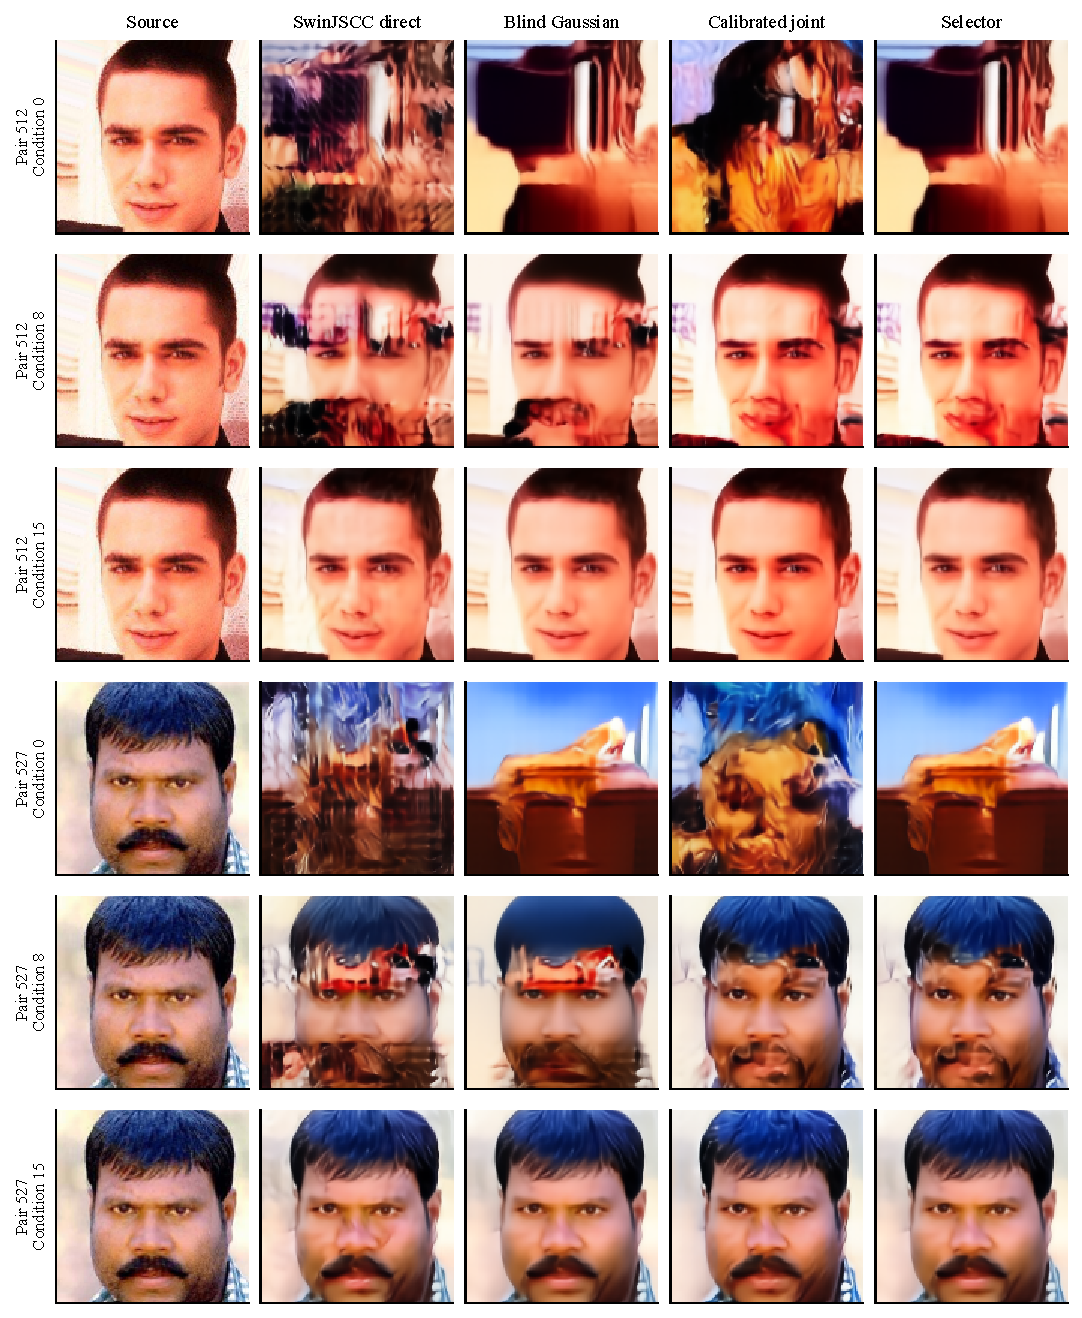
\includegraphics[width=\columnwidth]{figures/qualitative_prespecified.pdf}
\caption{All six qualitative examples reserved before confirmation: two image
pairs crossed with conditions 0, 8 and 15. The gallery is exhaustive for the
prespecified set and is not selected from observed reconstruction quality.}
\label{fig:qualitative}
\end{figure}

\section{Discussion and Conclusion}
In this paper, we proposed a blind selector that uses received energy and block-energy heterogeneity to choose between Gaussian denoising and joint signal--interference reconstruction with frozen neural weights. Independent confirmation shows PSNR gains of 0.750 and 1.334 dB over the respective receivers, with 34.7\% fewer predictor evaluations than joint sampling.

The gain is supported for the evaluated source, interference population and
inference budget. It is not a guarantee for individual frames: the harmful
tail persists, and block-boundary mismatch nearly removes the advantage over
Gaussian denoising. Received-energy heterogeneity can also originate from the
desired signal, so the branch label should be interpreted as a reconstruction
decision rather than identification of the interferer.

PSNR and MSE aggregate the same pixel errors differently; LPIPS and MS-SSIM
add perceptual evidence but do not measure success in a driving, recognition
or control task. Applying this receiver decision to vehicular communication
requires evaluation with task-specific losses, fading, channel estimation and
synchronization. The present results establish a narrower point: selecting
between existing disturbance models can improve average reconstruction while
reducing the cost of always invoking joint inference.
\bibliographystyle{IEEEtran}
\bibliography{references}
\end{document}
